\hypertarget{functionchap}{%
\section{Function calls}\label{functionchap}}

\index{función, llamada a}

In the programming context, a \emph{function} is a sequence of statements that perform an operation and are given a name. When a function is defined, the name and the sequence of statements are specified. Later, you can ``call'' the function by that name. We have already seen an example of a \emph{function call}:

\begin{Verbatim}[frame=single]
>>> type(32)
<class 'int'>
\end{Verbatim}


The function name is \pythoninline{type}. The expression in parentheses is called the \emph{argument} of the function. The argument is a value or variable that is passed to the function as an input parameter. The result of the \pythoninline{type} function is the type of the argument.

\index{paréntesis!argumento in}

It is common to say that a function ``takes'' (or receives) an argument and ``returns'' a result. The result is called \emph{value return}.

\index{argumento} \index{valor de retorno}

\section{Built-in functions)}\label{funciones-predefinidad}

Python provides a large number of built-in functions, which can be used without having to write them first. The creators of Python have written a set of functions to solve common problems and included them in Python for us to use.

The functions \pythoninline{max} and \pythoninline{min} will give us the largest and smallest value of a list, respectively:

\begin{Verbatim}[frame=single]
>>> max('Hello world!')
  'w'
>>> min('Hello world!')
  ' '
\end{Verbatim}

The \pythoninline{max} function tells us what the ``largest character'' in the string is (which is the letter ``w''), while the \pythoninline{min} function returns the smallest character (which in that case is a space). Remember that the string comparison uses the ASCII codes of the characters. These codes can be found using the predefined function \pythoninline{ord}:

\begin{Verbatim}[frame=single]
>>> ord(" ")
  32
>>> ord("a")
  97
>>> ord("u")
  117
>>> ord("H")
  72
>>> ord("!")
  33
\end{Verbatim}

Another very common built-in function is \pythoninline{len}, which tells us how many elements are in its argument. If the argument of \pythoninline{len} is a string, it returns the number of characters in the string.

\begin{Verbatim}[frame=single]
>>> len('Hello world!')
  12
>>>
\end{Verbatim}

These functions are not limited to strings. They can operate on any set of values, as we will see in the following chapters.

\begin{Verbatim}[frame=single]
>>> len([1,2,3,4,5]) #a list
  5
>>> len({1:"one", 2:"two", 3:"three"})  #a dictionary
  3
\end{Verbatim}

Predefined function names should be treated as if they were reserved words (i.e. avoid using \pythoninline{max} as a variable name).

\hypertarget{funciones-de-conversiuxf3n-de-tipos}{%
\section{Type conversion functions}\label{funciones-de-conversiuxf3n-de-tipos}}

\index{conversión!tipo} \index{tipo, conversión de}

Python also provides built-in functions that convert values from one type to another. The \pythoninline{int} function takes any value and converts it to an integer if it can, or complains if it can't:

\index{int, función} \index{función!int}

\begin{Verbatim}[frame=single]
>>> int('32')
  32
>>> int('Hello')
  ValueError: invalid literal for int() with base 10: 'Hello'
\end{Verbatim}

\pythoninline{int} can convert floating point values to integers, but does not round them; just cut and discard the decimal part:

\begin{Verbatim}[frame=single]
>>> int(3.99999)
  3
>>> int(-2.3)
  -2
\end{Verbatim}

\pythoninline{float} converts integers and strings to floating point numbers:

\index{float, función} \index{función!float}

\begin{Verbatim}[frame=single]
>>> float(32)
  32.0
>>> float('3.14159')
  3.14159
\end{Verbatim}

Finally, \pythoninline{str} converts its argument to a string:

\index{str, función} \index{función!str}

\begin{Verbatim}[frame=single]
>>> str(32)
  '32'
>>> str(3.14159)
'. 3.14159'
\end{Verbatim}

\hypertarget{funciones-matemuxe1ticas}{%
\section{Math functions (the math module))}\label{funciones-matemuxe1ticas}}

\index{math, función} \index{función!math} \index{módulo}
\index{módulo, objeto}

Python has a math module \texttt{(math)}, which provides most of the usual math functions. Before we can use the module, we need to import it:

\begin{Verbatim}[frame=single]
>>> import math
\end{Verbatim}

This statement creates a \emph{module object} called math. If you print the module object, you get some information about it:

\begin{Verbatim}[frame=single]
>>> print(math)
  <module 'math' (built-in)>
\end{Verbatim}

The module object contains the functions and variables defined in the module. To access one of those functions, you need to specify the module name and the function name, separated by a period. This format is called \emph{dot notation}.

\index{notación punto}

\begin{python}[frame=single]
import math

relation = 25
decibels = 10 * math.log10(relation)

radians = 0.7
height = math.sin(radians)
\end{python}

The first example computes the base 10 logarithm of a variable \pythoninline{relation}. The math module also provides a function called \pythoninline{log} that computes logarithms to the base \texttt{e}.

\index{log, función} \index{función!log} \index{sine, función}
\index{radián} \index{trigonométrica, función}
\index{función, trigonométrica}

The second example calculates the sine of the variable \pythoninline{radians}. The variable name is a hint that \pythoninline{sin} and the other trigonometric functions (\pythoninline{cos}, \pythoninline{tan}, etc.) take arguments in radians. To convert from degrees to radians, divide by 360 and multiply by \(2\pi\):


\pythonexternal{code/grados_a_radianes.py}


\begin{Verbatim}[frame=single]
>>> %Run 
  How many degrees do you want to convert to radians? 45
  45.0 degrees is 0.7071067811865475 radians
\end{Verbatim}

The expression \pythoninline{math.pi} takes the variable \pythoninline{pi} from the math module. The value of that variable is an approximation of \(\pi\), accurate to about 15 digits.

\index{pi}

\hypertarget{nuxfameros-aleatorios}{%
\section{Random numbers (the random module)}\label{nuxfameros-aleatorios}}

\index{aleatorio, número} \index{número, aleatorio}
\index{determinístico} \index{pseudoaleatorio}

From the same inputs, most programs will generate the same outputs every time, which is what we call \emph{deterministic} behavior. Determinism is usually a good thing, since we expect the same operation to always give us the same result. For certain applications, however, we will want the result to be unpredictable. Games are the obvious example, but there is more.

Making a program truly non-deterministic is not that easy, but there are ways to make it at least appear so. One of them is to use \emph{algorithms} that generate \emph{pseudo-random} numbers. Pseudo-random numbers are not truly random, since they are generated by a deterministic operation, but if we only look at the numbers it is almost impossible to distinguish them from truly random ones.

\index{random, módulo} \index{módulo!random}

The \texttt{random} module provides functions that generate pseudo-random numbers (which we will simply call ``random'' from now on).

\index{random, función} \index{función!random}

The \pythoninline{random} function returns a random float number between 0.0 and 1.0 (including 0.0, but not 1.0). Each time \pythoninline{random} is called, the next number in a long series is returned. To see an example, run this loop:

\begin{python}[frame=single]
import random

for i in range(10):
    x = random.random()
    print(x)
\end{python}

This program produces the following list of 10 random numbers between 0.0 and (but not including) 1.0.

\begin{Verbatim}[frame=single]
0.11132867921152356
0.5950949227890241
0.04820265884996877
0.841003109276478
0.997914947094958
0.04842330803368111
0.7416295948208405
0.510535245390327
0.27447040171978143
0.028511805472785867
\end{Verbatim}

As an exercise, test this program on your system and see what numbers you get.

The \pythoninline{random} function is just one of many that work with random numbers. The \pythoninline{randint} function takes the parameters \texttt{lower} and \texttt{upper}, and returns an integer between \texttt{lower} and \texttt{upper} (including both ends).

\index{randint, función} \index{función!randint}

\begin{Verbatim}[frame=single]
>>> random.randint(5, 10)
  5
>>> random.randint(5, 10)
  9
\end{Verbatim}

To choose an element from a sequence randomly, \pythoninline{choice} can be used:

\index{choice, función} \index{función!choice}

\begin{Verbatim}[frame=single]
>>> random.choice([1, 2, 3])
  2
>>> random.choice("hello world")
  'l'
\end{Verbatim}

The \texttt{random} module also provides functions to generate random values from various continuous distributions, including Gaussian, exponential, gamma, and a few more.

\hypertarget{auxf1adiendo-funciones-nuevas}{%
\section{Adding new features}\label{auxf1adiendo-funciones-nuevas}}

So far, we have only been using the built-in functions of Python, but it is possible to add new functions as well. A \emph{function definition} specifies the name of a new function and the sequence of statements that are executed when that function is called. Once a function is defined, it can be reused over and over again throughout the program.

\index{función} \index{función, definición} \index{definición!función}

Here's an example:

\begin{python}[frame=single]
def sample_chorus():
    print("I said maybe")
    print("You're gonna be the one that saves me")
    print("And after all")
    print("You're my wonderwall")
\end{python}

\pythoninline{def} is a keyword indicating that this is a function definition. The name of the function is \pythoninline{sample\_chorus}. The rules for function names are the same as for variables: letters, numbers, and some punctuation marks can be used, but the first character cannot be a number. You can't use a keyword as a function name, and you should also avoid having a variable and a function
with the same name.

\index{def, palabra clave} \index{palabra clave!def} \index{argumento}

Empty parentheses after the name indicate that this function takes no arguments. Later we will build functions that receive input parameters.

\index{paréntesis!vacíos} \index{cabecera} \index{cuerpo}
\index{indentado} \index{dos-puntos}

The first line of the function definition is called the \emph{header}; the rest is called the \emph{body}. The header must end with a colon (:), and the body must be indented. By convention, the indent is always four spaces. The body can contain any number of statements. The different parts of the functions can be seen in Figure \ref{fig:partes_funciones}.

\begin{figure}[t]
    \centering
    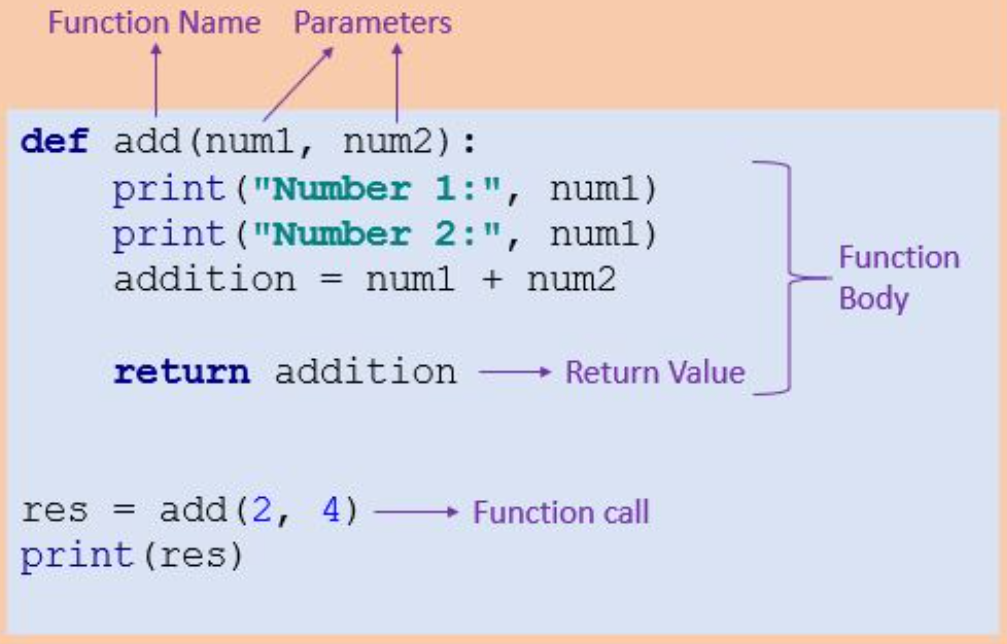
\includegraphics[width=\0.75\textwidth]{images/funciones_partes-eng.png}
    \caption{Functions in python}
    \label{fig:partes_funciones}
\end{figure}


\index{puntos suspensivos}
If you write a function definition in interactive mode in the console, the interpreter will display ellipses (\emph{\ldots{}}) to inform you that the definition is not complete:

\begin{Verbatim}[frame=single]
>>> def sample_chorus():
...     print("I said maybe")
...     print("You're gonna be the one that saves me")
...     print("And after all")
...     print("You're my wonderwall")
\end{Verbatim}

To end the function, you must enter an empty line (this is not necessary in a script).

When defining a function, a variable with the same name is created.

\begin{Verbatim}[frame=single]
>>> print(sample_chorus)
  <function sample_chorus at 0xb7e99e9c>
>>> print(type(sample_chorus))
  <type 'function'>
\end{Verbatim}

The value of \pythoninline{sample\_chorus} is \emph{function object}, which has type ``function''.

\index{función, objeto} \index{objeto!función}

The syntax for calling our new function is the same as we use for predefined functions:

\begin{Verbatim}[frame=single]
>>> sample_chorus()
  I said maybe
  You're gonna be the one that saves me
  And after all
  I said, I bet that you look good on the dance floor
\end{Verbatim}

Once a function has been defined, it can be used inside another. For example, to repeat the previous chorus, we could write a function called \pythoninline{repeat\_chorus}:

\begin{python}[frame=single]
def repeat_chorus():
    sample_chorus()
    sample_chorus()
\end{python}

And then call \pythoninline{repeat\_chorus}:

\begin{Verbatim}[frame=single]
>>> repeat_chorus()
  I said maybe
  You're gonna be the one that saves me
  And after all
  You're my wonderwall
  I said maybe
  You're gonna be the one that saves me
  And after all
  You're my wonderwall
\end{Verbatim}


\hypertarget{definiciuxf3n-y-usos}{%
\section{Definition and uses}\label{definiciuxf3n-y-usos}}

\index{función, definición}

Putting the code snippets from the previous sections together, the complete program would look something like this:

\begin{python}[frame=single]
def sample_chorus():
    print("I said maybe")
    print("You're gonna be the one that saves me")
    print("And after all")
    print("You're my wonderwall")

def repeat_chorus():
    sample_chorus()
    sample_chorus()

repeat_chorus()
\end{python}

This program contains two function definitions: \pythoninline{sample\_chorus} and \pythoninline{repeat\_chorus}. Function definitions are executed just like any other statement, but their result is to create objects of type function. Statements within each function are executed only when that function is called, and a function definition does not generate any output.

\index{use before def}

As you can imagine, it is necessary to create a function before it can be executed. In other words, the function definition must be executed before the function is called for the first time.

Shift the last line of the above program up, so that the function call appears before the definitions. Run the program and see what error message you get.

Move the function call back to the end, and put the \pythoninline{sample\_chorus} definition after the \pythoninline{repeat\_chorus} definition. What happens when you try that program?

\hypertarget{flujo-de-ejecuciuxf3n}{%
\section{Execution flow}\label{flujo-de-ejecuciuxf3n}}

\index{flujo de ejecución}

To make sure that a function is defined before using it for the first time, it is necessary to know the order in which the statements are executed, which is what we call the \emph{execution flow}.

Execution always starts at the first statement in the program. The statements are executed one by one, in order from top to bottom.

Function \emph{definitions} do not alter the flow of program execution, but remember that statements within a function are not executed until that function is called.

A function call is like a detour in the flow of execution. Instead of going to the next statement, the stream jumps to the body of the function, executes all the statements there, and then returns to where it left off.

This all sounds pretty straightforward, until you remember that one function can call another. When in the middle of a function, the program may have to execute the statements of another function. But when you're executing that new function, there may be even more functions to execute!

Fortunately, Python is able to keep track of where it is at any given moment, so that each time it completes a function's execution, the program returns to where it left off in the function that called it. When this takes you to the end of the program, it just ends.

What is the moral of this strange story? When you read a program, you don't always want to do it from top to bottom. Sometimes it makes more sense to go with the flow of execution.

\hypertarget{paruxe1metros-y-argumentos}{%
\section{Parameters and arguments}\label{paruxe1metros-y-argumentos}}

\index{parámetro} \index{parámetro!de función} \index{argumento}
\index{argumento de función}

Some of the built-in functions we've seen need arguments. For example, when \pythoninline{math.sin} is called, it is passed a number as an argument. Some functions need more than one argument: \pythoninline{math.pow} takes two, the base and the exponent.

Inside functions, the arguments are assigned to variables called \emph{parameters}. Here's an example of a user-defined function that takes one argument:

\index{paréntesis!parámetros entre}

\begin{python}[frame=single]
def show_twice(bruce):
    print(bruce)
    print(bruce)
\end{python}

This function assigns the argument to a parameter named \pythoninline{bruce}. When the function is called, it prints the value of the parameter (whatever it is) twice.

This function works with any value that can be displayed on the screen.

\begin{Verbatim}[frame=single]
>>> show_twice('Spam')
  Spam
  Spam
>>> show_twice(18)
  18
  18
>>> show_twice(math.pi)
  3.14159265359
  3.14159265359
\end{Verbatim}

The same composition rules that apply to built-in functions also apply to user-defined functions, so we can use any type of expression as an argument to \pythoninline{display\_twice\_times}:

\index{composición}

\begin{Verbatim}[frame=single]
>>> show_twice('Spam '*4)
  Spam Spam Spam Spam
  Spam Spam Spam Spam
>>> show_twice(math.cos(math.pi))
  -1.0
  -1.0
\end{Verbatim}

The argument is evaluated before the function is called, so in the examples, the expression \texttt{Spam\ *4} and \pythoninline{math.cos(math.pi)} are evaluated only once.

\index{argumento}

A variable can also be used as an argument:

\begin{Verbatim}[frame=single]
>>> michael = 'Maya the bee.'
>>> show_twice(michael)
  Maya the bee.
  Maya the bee.
\end{Verbatim}

The name of the variable that we pass as an argument, (\texttt{michael}) has nothing to do with the name of the parameter (\texttt{bruce}). It doesn't matter how the value was called at the source (in the call); inside \texttt{show\_twice}, it will always be called \texttt{bruce}.

\hypertarget{funciones-productivas-y-funciones-estuxe9riles}{%
\section{Fruitful functions and void functions}\label{funciones-productivas-y-funciones-estuxe9riles}}

\index{productiva, función} \index{estéril, función}
\index{función productiva} \index{función esteril}

Some of the functions we're using, like math, produce results; For lack of a better name, we'll call them \emph{fruitful functions}. Other functions, like \pythoninline{show\_twice}, perform an action, but do not return a value. We will call these \emph{void functions}.

When you call a fruitful function, you almost always want to do something with the result afterwards; for example, you may want to assign it to a variable or use it as part of an expression:

\begin{python}[frame=single]
x = math.cos(radians)
aurea = (math.sqrt(5) + 1) / 2
\end{python}

When you call a function in interactive mode, Python displays the result:

\begin{Verbatim}[frame=single]
>>> math.sqrt(5)
  2.23606797749979
\end{Verbatim}

But in a script, if you call a fruitful function and don't store the result of it in a variable, the return value vanishes into mist!

\begin{python}[frame=single]
math.sqrt(5)
\end{python}

This script calculates the square root of 5, but since it doesn't store the result in a variable or display it, it's not really very useful.

\index{interactivo, modo} \index{script, modo}

Void functions can display something on the screen or have any other effect, but they don't return a value. If you try to assign the result to a variable, you will get a special value called \pythoninline{None} (nothing).

\index{None, valor especial} \index{valor especial!None}

\begin{Verbatim}[frame=single]
>>> result = show_twice('Bing')
  Bing
  Bing
>>> print(result)
None
\end{Verbatim}

Remember, the value \pythoninline{None} is not the same as the string ``None''. It is a special value that has its own type:

\begin{Verbatim}[frame=single]
>>> print(type(None))
  <class 'NoneType'>
\end{Verbatim}

To return a result from a function, we use the \pythoninline{return} statement within it. For example, we can create a very simple function called \pythoninline{add_nums}, which adds two numbers together and returns the result.

\begin{python}[frame=single]
def add_nums(a, b):
    sum = a + b
    return sum

x = add_nums(3, 5)
print(x)
\end{python}

When this script is run, the \texttt{print} statement will return ``8'', since the \pythoninline{add_nums} function has been called with 3 and 5 as arguments. Inside the function, the parameters \pythoninline{a} and \pythoninline{b} will equal 3 and 5 respectively. The function calculated the sum of both numbers and stored it in a variable local to the function called \pythoninline{sum}. It then used the \pythoninline{return} statement to send the calculated value back to the calling code as the result of the function, which was assigned to the variable \pythoninline{x} and displayed on the screen.

\hypertarget{por-quuxe9-funciones}{%
\section{Why functions?}\label{por-quuxe9-funciones}}


\index{función, razones para}

It may not be very clear why it is worth bothering to break a program into functions. There are several reasons:

\begin{itemize}
\item
  Creating a new function gives you the opportunity to name a group of statements, which makes your program easier to read, understand, and debug.
\item
  Functions can make a program smaller by eliminating duplicate code. Also, if you want to make any changes in the future, you only have to do it in one place.
\item
  Breaking a long program into functions allows you to debug the parts one at a time and then assemble them together into one piece.
\item
  Well-designed functions are often useful for many other programs. Once you've written and debugged one, you can reuse it.
\end{itemize}

We can see these things for example in Figure \ref{fig:sin.con.funciones} where you can compare 2 equivalent programs: one that uses functions and the other doesn't.

\begin{figure}[H]
    \centering
    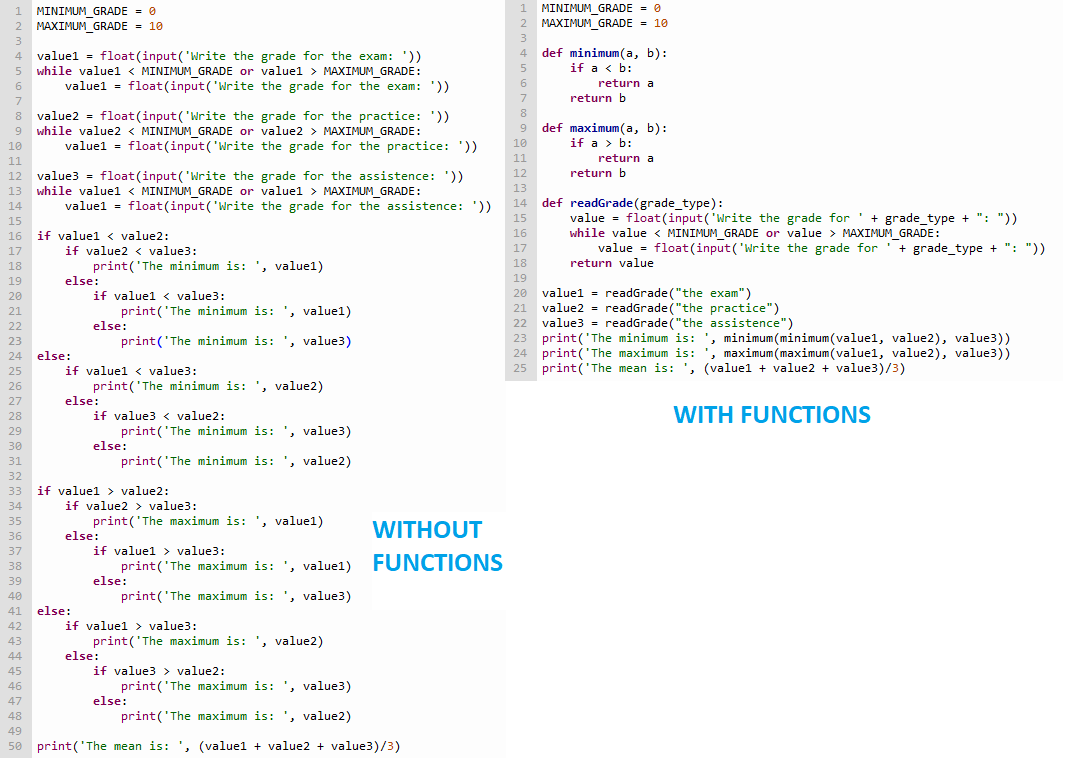
\includegraphics[width=0.90\textwidth]{images/sin-con-funciones-eng.png}
    \caption{Comparison of a program without and with functions}
    \label{fig:sin.con.funciones}
\end{figure}


\section{docstring}
\label{docstring}
\index{docstring}

A {\bf docstring} is a string at the beginning of a function that explains what the function can be used for (``doc'' is short for ``documentation''). Here is an example:

\begin{python}
def minimum(a, b):
    """
    Returns the minimum of the two given numbers.
    """
    if a > b:
        return a
    return b
\end{python}
%
By convention, all docstrings are triple-quoted strings, also known as multiline strings because triple quotes allow the string to be expanded to more than one line.
\index{comillas}
\index{cadena!entre triple comillas}
\index{triple comillas, cadena entre}
\index{cadena!multilínea}
\index{multilínea, cadena}

It's short, but it contains the essential information someone would need to use this feature. It concisely explains what the function does (without going into detail about how it does it). Explain what effect each parameter has on the function's behavior and what type each parameter should be (if it's not obvious).

Writing this type of documentation is an important part of designing the feature. A well-designed function should be simple to explain; If you're having trouble explaining one of your features, perhaps the interface could use some improvement.

Docstrings are accessible with the built-in \pythoninline{help} function.

\begin{Verbatim}[frame=single]
>>> help(minimum)
Help on function minimum in module __main__:

minimum(a, b)
    Returns the minimum of the two given numbers.
\end{Verbatim}






\section{Testing our functions (the pytest module)}


We already know that all the programs we write must be tested to check that the results of our programs match what we expect.
%
When we write programs that we can interact with via the console, we can test our program by entering test input data via the keyboard and checking the resulting output on the screen.
%
However, now when we write functions, we can use the \pythoninline{pytest} module to test their operation.

For example, imagine that we have to write a function \pythoninline{no_vowels} that, given a string \pythoninline{s}, returns the same string \pythoninline{s} but without vowels. For example:

\begin{Verbatim}[frame=single, label = {\em example of execution}]
>>> no_vowels("the water is wet")
  th wtr s wt
\end{Verbatim}

What tests would you run to test your program well? We can try with:

\begin{itemize}[nosep]
    \item the example string \texttt{''the water is wet''}, 
    \item the example starts with a consonant, let's do another test that starts with a vowel
    \item the example ends with a consonant, let's do another test that ends with a vowel
    \item a string that starts and ends with a vowel
    \item the empty string,
     \item a string without spaces,
    \item a string with only one vowel letter,
     \item a string with only one consonant letter,
    \item a string with capital letters
    \item a string that has no vowels
    \item a string that only has vowels
    \item a string with digits
    \item a string with question marks and others
\end{itemize}

We design our test suite by choosing expected input and output values:

\begin{tabular}{|l|l|l|l|}
\hline
test case & input & expected output & comment  \\ \hline\hline
1 & \verb@"the water is wet"@ & \verb@"th wtr s wt"@ & the example string\\
2 & \verb@"is wet the water"@ & \verb@"s wt th wtr"@ & starts with a vowel\\
3 & \verb@"new sentence"@ & \verb@"nw sntnc"@ & ends with a vowel\\
4 & \verb@"another sentence"@ & \verb@"nthr sntnc"@ & ends with a vowel\\
5 & \verb@""@ & \verb@""@ & the empty string\\
6 & \verb@"a"@ & \verb@""@ & only one vowel letter\\
7 & \verb@"m"@ & \verb@"m"@ & only one consonant letter\\
8 & \verb@"astringwithoutspaces"@ &  \verb@"strngwthtspcs"@ & without spaces\\
9 & \verb@"CAPITal letTERS wORk"@ & \verb@"CPTl ltTRS wRk"@ & string with capital letters\\
10 & \verb@"krt yhgf dwpq"@ & \verb@"krt yhgf dwpq"@ & has no vowels\\
11 & \verb@"aeoiuuuoiea"@ & \verb@""@ & only has vowels\\
12 & \verb@"album released in the 80s"@ & \verb@"lbm rlsd n th 80s"@ & with digits\\
13 & \verb@"marks like ? and !"@ & \verb@"mrks lk ? nd !"@ & with question marks and others\\
\hline
\end{tabular}

Imagine that we implement our function in a file called \texttt{no\_vowels.py}

\begin{python}
def no_vowels (s):
    """
    returns the argument s without vowels
    """
    vowels = 'aeiouAEIOU'
    s_noVowels = ''
    for ch in s:
        pos = vowels.find(ch)
        if pos == -1: #ch is not vowel
            s_noVowels = s_noVowels + ch     
    return s_noVowels
\end{python}

We can now run the above tests automatically with pytest, defining:

\begin{python}
import pytest

@pytest.mark.parametrize("test_case, input, expected_output",[
(1, "the water is wet", "th wtr s wt"),             #string example
(2, "astringwithoutspaces", "strngwthtspcs"),       #without spaces
(3, "", ""),                                        #the empty string
(4, "CAPITal letTERS wORk", "CPTl ltTRS wRk"),      #string with capital letters
(5, "krt yhgf dwpq", "krt yhgf dwpq"),              #has no vowels
(6, "aeoiuuuoiea", ""),                             #only has vowels
(7, "album released in the 80s", "lbm rlsd n th 80s"),     #with digits
(8, "marks like ? and !", "mrks lk ? nd !")         #with question marks and others
])

def test_no_vowels(test_case, input, expected_output):
    assert no_vowels(input) == expected_output, "case {0}".format(test_case)
\end{python}

The \pythoninline{pytest.mark.parametrize} allows us to define the test cases (i.e. the expected inputs and outputs) that we want to execute. The first argument to \pythoninline{pytest.mark.parametrize}, ie: \pythoninline{'case_num, input, expected_output'}, reflects the components of the test cases for this function. This is called \emph{test signature} and for this function it matches the first 3 columns of our table above.

\begin{itemize}
    \item \pythoninline{'test_case '}: the identifier/number of the test
    \item \pythoninline{'input'}: the input we want to give to the function
    \item \pythoninline{'expected_output'}: the output we expect to come out
\end{itemize}

The rest of the arguments to \pythoninline{pytest.mark.parametrize} consist of the test cases we have defined.

We then define a test function \pythoninline{test_vowelless} that takes a number of parameters that matches the \emph{test signature}. The only thing the function does is:
\begin{itemize}
    \item call the function we want to test with the inputs \pythoninline{no_vowels(input)}
    \item compare output to expected output \pythoninline{== expected_output}
    \item when the \pythoninline{assert} statement receives a \pythoninline{True} (meaning that the output of the function is what we expected) it does nothing.
    \item when the \pythoninline{assert} instruction receives a \pythoninline{False} (which means that what we expected did NOT come out) then it throws a message indicating that the test case (\pythoninline{case_num}) has failed.
\end{itemize}


The \pythoninline{pytest} module ensures that the test function receives all test cases defined in \pythoninline{pytest.mark.parametrize}. To run the tests we do in the Thonny console:


\begin{Verbatim}[frame=single]
>>> !py.test no_vowels.py
============================= test session starts ==============================
platform darwin -- Python 3.7.9, pytest-6.1.2, py-1.9.0, pluggy-0.13.1
rootdir: /Users/tanjavos/Python/Tema5
collected 8 items

no_vowels.py ........                                                    [100%]
============================== 8 passed in 0.02s ===============================
\end{Verbatim}
    
And we see that the 8 test cases that we have defined have passed. Our program has survived all 8 tests!


\section{CODS, a mnemonic for testing}\label{test-mnemonic}
\index{mnemonic}

To have a little more guidance on what test cases to test with your program, we can use the CODE mnemonic:

\begin{description}
\item[{\color{red} C}]ardinality
\item[{\color{red} O}]rder
\item[{\color{red} D}]omain
\item[{\color{red} E}]ach structure
\end{description}

This mnemonic is inspired by Jeff Langr's book, {\em Pragmatic Unit Testing in Java 8 with JUnit}. The words that make up the mnemonic can help us generate ideas as to which entries to try, just that. It's not guaranteed to come up with ideas, nor does it apply to all possible features, but it's always helpful to be able to start with something that can spark ideas for you.

\subsection{{\color{red} C}ardinality}

In mathematics, the cardinality of a value is the measure of the "number of elements". For example, the string \pythoninline{'abcd'} contains 4 letters, and therefore has cardinality 4. This part of the mnemonic reminds us to try different cardinalities of the inputs. For example,

\begin{itemize}
    \item cardinality 0
    \item cardinality 1
    \item cardinality > 1
\end{itemize}

We recall the function \pythoninline{no_vowels} that given a string \pythoninline{s}, returns the same string \pythoninline{s} but without vowels.

\begin{Verbatim}[frame=single, label = {\em example of execution}]
>>> no_vowels("the water is wet")
  th wtr s wt
\end{Verbatim}

Among the test cases that we saw before, the ones that check different cardinalities for s are:

\begin{tabular}{|l|l|l|l|}
\hline
test case & input & expected output & comment  \\ \hline\hline
1 & \verb@"the water is wet"@ & \verb@"th wtr s wt"@ & cardinality \pythoninline{s} > 1\\
4 & \verb@""@ & \verb@""@ & the empty string, cardinality \pythoninline{s} = 0\\
5 & \verb@"a"@ & \verb@""@ & cardinality \pythoninline{s} = 1, only one vowel letter\\
6 & \verb@"m"@ & \verb@"m"@ & cardinality \pythoninline{s} = 1, only one consonant letter\\
\hline
\end{tabular}


\subsection{{\color{red} O}rder}

For some functions and their solutions, the order of elements is important, for others it is not. In both cases, it is necessary to prove that the method works well.

We recall the function \pythoninline{no_vowels} that given a string \pythoninline{s}, returns the same string \pythoninline{s} but without vowels.

Among the test cases we saw earlier, the ones that check different order of where the vowels are for \pythoninline{s} are:

\begin{tabular}{|l|l|l|l|}
\hline
test case & input & expected output & comment  \\ \hline\hline
1 & \verb@"the water is wet"@ & \verb@"th wtr s wt"@ & starts and ends with consonant\\
2 & \verb@"another sentence"@ & \verb@"nthr sntnc"@ & starts and ends with vowel\\
3 & \verb@"new sentence"@ & \verb@"nw sntnc"@ & starts with a consonant\\
4 & \verb@"is wet the water"@ & \verb@"s wt th wtr"@ & ends with a consonant\\
\hline
\end{tabular}

\subsection{{\color{red} D}omain}

You have to think about whether it is necessary to try different domains of the parameters and their limits.

The specification of the function \pythoninline{no_vowels} clearly says that it has to work when given an argument of type string \pythoninline{s}. So it doesn't really need to work for types int, float, etc. because it is not what the function promises. What we can do is try with strings that contain numbers, to verify that our function works and does not, for example, detect it as vowels or something like that.

Among the test cases we saw earlier, the ones that check for different order of where the vowels are for \pythoninline{s} are:

\begin{tabular}{|l|l|l|l|}
\hline
test case & input & expected output & comment  \\ \hline\hline
11 & \verb@"album released in the 80s"@ & \verb@"lbm rlsd n th 80s"@ & with digits\\
\hline
\end{tabular}


\subsection{{\color{red} E}ach structure}

The structure of the parameters can be very important for the good behavior  of a function. We see that for the function \pythoninline{no_vowels} and the argument \pythoninline{s} of type String, the rest of the test cases that we saw before check different structures of the string \pythoninline{s}:

\begin{tabular}{|l|l|l|l|}
\hline
test case & input & expected output & comment  \\ \hline\hline
7 & \verb@"astringwithoutspaces"@ &  \verb@"strngwthtspcs"@ &  without spaces\\
8 & \verb@"CAPITal letTERS wOR"@ & \verb@"CPTl ltTRS wR"@ &  string with capital letters\\
9 & \verb@"krt yhgf dwpq"@ & \verb@"krt yhgf dwpq"@ & has no vowels\\
10 & \verb@"aeoiuuuoiea"@ & \verb@""@ & only has vowels\\
12 & \verb@"marks like ? and !"@ & \verb@"mrks lk ? nd !"@ & with question marks and others\\
\hline
\end{tabular}





\hypertarget{editor}{%
\section{Debugging}\label{editor}}

\index{depuración}

If you are using a text editor to write your own scripts, you may have problems with spaces and tabs. The best way to avoid these problems is to use spaces exclusively (no tabs). Most text editors that recognize Python do so by default, although there are a few that don't.

\index{espacio en blanco}

Tabs and spaces are usually invisible, which makes it difficult to debug any errors that may occur, so find an editor that handles the indenting for you.

Also don't forget to save your program before running it. Some development environments do this automatically, but others don't. In that case, the program you're seeing in the text editor may not be the one you're actually running.

Debugging can take a long time if you're running the same buggy program over and over again!

Make sure the code you're examining is the same code you're executing. If you're not sure, put something like \texttt{print("hello")} at the top of the program and run it again. If you don't see \texttt{hello} on the screen, you're not running the right program!

\hypertarget{glosario}{%
\section{Glossary}\label{glosario}}

\begin{description}
\item[algorithm]
A general process for solving a category of problems.
\end{description}
\index{algoritmo}

\begin{description}
\item[argument]
A value provided to a function when it is called. That value is assigned to the corresponding parameter in the function.
\end{description}
\index{argumento}

\begin{description}
\item[body]
The sequence of statements within a function definition.
\end{description}
\index{cuerpo}

\begin{description}
\item[composition]
Using an expression or statement as part of a longer one.
\end{description}
\index{composición}

\begin{description}
\item[deterministic]
Pertaining to a program that does the same thing each time it is run, from the same inputs.
\end{description}
\index{determinístico}

\begin{description}
\item[dot notation]
The syntax for calling a function from another module, specifying the module name followed by a dot and the function name.
\end{description}
\index{punto, notación}

\begin{description}
\item[execution flow]
The order in which statements are executed during the operation of a program.
\end{description}
\index{flujo de ejecución}

\begin{description}
\item[fruitful function]
A function that returns a value.
\end{description}
\index{productiva, función}

\begin{description}
\item[function]
A sequence of named statements that perform some useful operation. Functions may or may not take arguments, and may or may not produce a result.
\end{description}
\index{función}

\begin{description}
\item[function call]
A statement that executes a function. It consists of the function name followed by a list of arguments.
\end{description}
\index{función, llamada a}

\begin{description}
\item[function definition]
A statement that creates a new function, specifying its name, parameters, and the statements it executes.
\end{description}
\index{función, definición}

\begin{description}
\item[function object]
A value created by a function definition. The function name is a variable that refers to the function object.
\end{description}
\index{función, definición}

\begin{description}
\item[header]
The first line of a function definition.
\end{description}
\index{cabecera}

\begin{description}
\item[import sentence]
A statement that reads a module file and creates a module object.
\end{description}
\index{import, sentencia} \index{sentencia!import}

\begin{description}
\item[module object]
A value created by an \texttt{import} statement, which provides access to the data and code defined in a module.
\end{description}
\index{módulo}

\begin{description}
\item[parameter]
A name used inside a function to refer to the value passed as an argument.
\end{description}
\index{parámetro}

\begin{description}
\item[pseudo-random]
Pertaining to a sequence of numbers that appear to be random, but are generated by a deterministic program.
\end{description}
\index{pseudoaleatorio}

\begin{description}
\item[return value]
The result of a function. If a function call is used as an expression, the return value is the value of the expression.
\end{description}
\index{valor de retorno}

\begin{description}
\item[void function]
A function that does not return any value.
\end{description}
\index{estéril, función}

